\chapter{Anharmonischer Oszillator\label{chapter:anharmonisch}}
\lhead{Anharmonischer Oszillator}
\begin{refsection}
\chapterauthor{Joel Brunner und Christian Cavegn}

\newpage
\section{Einleitung}
\rhead{Einleitung}
In diesem Kapitel erweitern wir den harmonischen Oszillator aus Kapitel 8 mit Hilfe der St"orungstheorie aus Kapitel 10. Der harmonische Oszillator ist eine gute Approximation f"ur viele Quantenmechanische Systeme. Will man die Approximation verbessern, kann man die Kräfte im Oszillator nicht mehr linear modellieren. Das Potential ist also nicht mehr nur $Q^2$, sondern es kommen noch Terme h"oherer Ordnung hinzu. Diese Terme können als St"orungen betrachtet werden.

\section{Anharmonizit"at}
\rhead{Anharmonizit"at}

\begin{figure}[h]	%Bild Potentiale
\centering
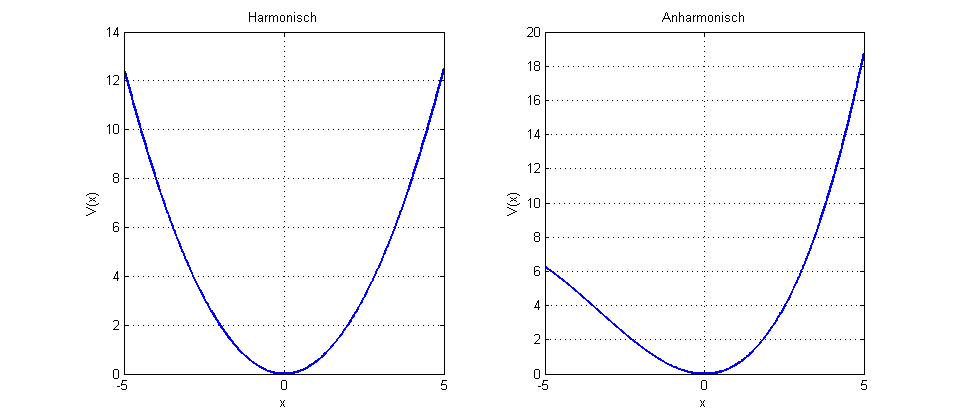
\includegraphics[width=0.7\textwidth]{anharmonisch/images/Potential.png}
\caption{Potentiale eines harmonischen und anharmonischen Oszillators
\label{skript:Potentiale}}
\end{figure}

Auf der Abbildung~\ref{skript:Potentiale} sieht man links das Potential des harmonischen Oszillators. Das System ist linear und wurde in Kapitel 8 vollständig gelöst. Rechts sieht man das Potential des gest"orten Oszillators. In diesem Fall sind zus"atzlich noch Terme wie $aQ^3$ oder $bQ^4$ im Potential enhalten. Der harmonische Term ist aber immer noch der dominierende.

\section{Harmonische Gr"ossen}
\rhead{Harmonische Gr"ossen}

\subsection{Wellenfunktionen}
Der Grundzustand (\ref{skript:grundzustandwellenfunktion}) hat die Form einer Gauss-Kurve. Mit der geeigneten Normierung bekommen wir den Grundzustand
\[
\Psi_0(x)
=
\biggl(\frac{m\omega}{\pi\hbar}\biggr)^\frac14
e^{-\frac12\frac{m\omega}{\hbar}x^2}
\]
Mit der Formel (\ref{eq:8.10}) wird eine eingache Iterationsfunktion Abgeleitet.
\[
\Psi_k(x)
=
\frac1{\sqrt{k!}}\biggl(\frac1{\sqrt{2}}
\biggl(\sqrt{\frac{m\omega}{\hbar}x}-
\sqrt{\frac{\hbar}{m\omega}}\frac{\partial}{\partial x}\biggr)\biggr)^k
\biggl(\frac{m\omega}{\pi\hbar}\biggr)^\frac14
e^{-\frac12\frac{m\omega}{\hbar}x^2}
\]
In die Gleichung substituiert man
\[
\alpha=\sqrt{\frac{m\omega}\hbar}
\]
und formt sie ein wenig um.
\[
\Psi_k(x)
=
\frac1{\sqrt{k!}}\frac1{\sqrt{2^k}}
\biggl(\frac{m\omega}{\pi\hbar}\biggr)^\frac14
\biggl(\alpha x-\frac1{\alpha}\frac{\partial}{\partial x}\biggr)^k
e^{-\frac12\alpha^2x^2}
\]
Durch ausmultiplizieren erhaltet man die entsprechende Wellenfunktion
\[
\biggl(\alpha x-\frac1{\alpha}\frac{\partial}{\partial x}\biggr)^1
e^{-\frac12\alpha^2x^2}
=
(2\alpha x)e^{-\frac12\alpha^2x^2}
\]
\[
\biggl(\alpha x-\frac1{\alpha}\frac{\partial}{\partial x}\biggr)^2
e^{-\frac12\alpha^2x^2}
=
\biggl(\alpha x-\frac1{\alpha}\frac{\partial}{\partial x}\biggr)
(2\alpha x)e^{-\frac12\alpha^2x^2}
=
\biggl(2\alpha^2 x^2-2\frac{\partial}{\partial x}x\biggr)
e^{-\frac12\alpha^2x^2}
\]
\[
(2\alpha^2x^2-(2-2\alpha^2x^2))e^{-\frac12\alpha^2x^2}
=
(4\alpha^2x^2-2)e^{-\frac12\alpha^2x^2}
\]
Man erh"alt die charakteristischen Hermitpolynome $H_k$,welche wir mit folgender Gleichung erhalten werden k"onnen.
\[
H_k(z)
=
e^{\frac{z^2}2}\biggl(z-\frac{\partial}{\partial z}\biggr)^k
e^{-\frac{z^2}2}.
\]
Dadurch wird die Gleichung gek"urzt zu
\[
Phi_k(z)
=
\biggl(\frac{m\omega}{\pi\hbar}\biggr)^\frac14
\frac1{\sqrt{2^k k!}}H_k(z)
e^{-\frac12 z^2}
\]
Das Hamilton Polynom lässt sich mit folgender Differeintialgleichung berechnen.
\[
H_k(x)
=
(-1)^k e^{x^2}\frac{\mathrm d^n}{\mathrm d x^n}
e^{-x^2},
\]
Der Vorteil dieser Notation ist die sehr einfache Implementierung in den g"angigen Berechunugstools\\
\\
Beispiele Retourwerte\\
TODO

\subsection{Energielevel}
\[
E_n
=
\hbar\omega\biggl(n+\frac12\biggr)
\]
Funktion\\
Beispiele Retourwerte TODO

\subsection{Störungstheorie}
Schr"odingergleichung in der St"orungstheorie
\[
(H_0+\varepsilon H_1)|\Psi_k(\varepsilon)\rangle
=
E_k(\varepsilon)|\Psi_k(\varepsilon)\rangle
\]
Koeffizienten
\[
E_k(\varepsilon)
=
E_k^{(0)}+\varepsilon E_k^{(1)}+\varepsilon^2 E_k^{(2)}+\dotsb
\]
\[
|\Psi_k(\varepsilon)\rangle
=
|\Psi_k^{(0)}\rangle+\varepsilon|\Psi_k^{(1)}\rangle+
\varepsilon^2|\Psi_k^{(2)}\rangle+\dotsb
\]
Durch geeignetes ausmultiplizieren wie in \ref{section:nichtentartetezustaende}  beschrieben kommt man auf folgende generische Gleichung:
\[
\langle\Psi_l^{(0)}|\Psi_k^{(p)}\rangle
=
\frac{C_{lk}^{p}-\langle\Psi_l^{(0)}|H_1|\Psi_k^{(k)}\rangle}
{E_l^{(0)}-E_k^{(0)}}
\]
\[
E_k^{(p)}
=
\langle\Psi_l^{(0)}|H_1|\Psi_l^{(k)}\rangle-C_{lk}^{(p)}
\]
mit
\[
C_{lk}^{(p)}
=
\displaystyle\sum_{j=2}^{p} E_k^{(p-j-1)}
\langle\Psi_l^{(0)}|\Psi_k^{(j-1)}\rangle
\]
Diese k"onnen einfach Implementiert werden\\
Code TODO\\
\\
Das Skalarprodukt beschreibt die Abh"angigkeit zweier Vektoren. Um sich eine bessere Vorstellung zu verschaffen dient folgende Gleichung
\[
\langle\Psi_l^{(0)}|\Psi_k^{(p)}\rangle^2
=
P\langle\Psi_l^{(0)}|\Psi_l^{(p)}\rangle
\]
Wie Wahrscheinlich ist es, dass die ungest"orte Wellenfunktion $|\Psi_l^{(0)}\rangle$ in der Zustandskorrektur $|\Psi_k^{(p)}\rangle$ vorkommt. In Abbildung~\ref{skript:PLK12} werden die Skalare der Wellenfunktionen 0 bis 50 dargestellt.

\begin{figure}[h]	%Bild PLK12.pdf
\centering
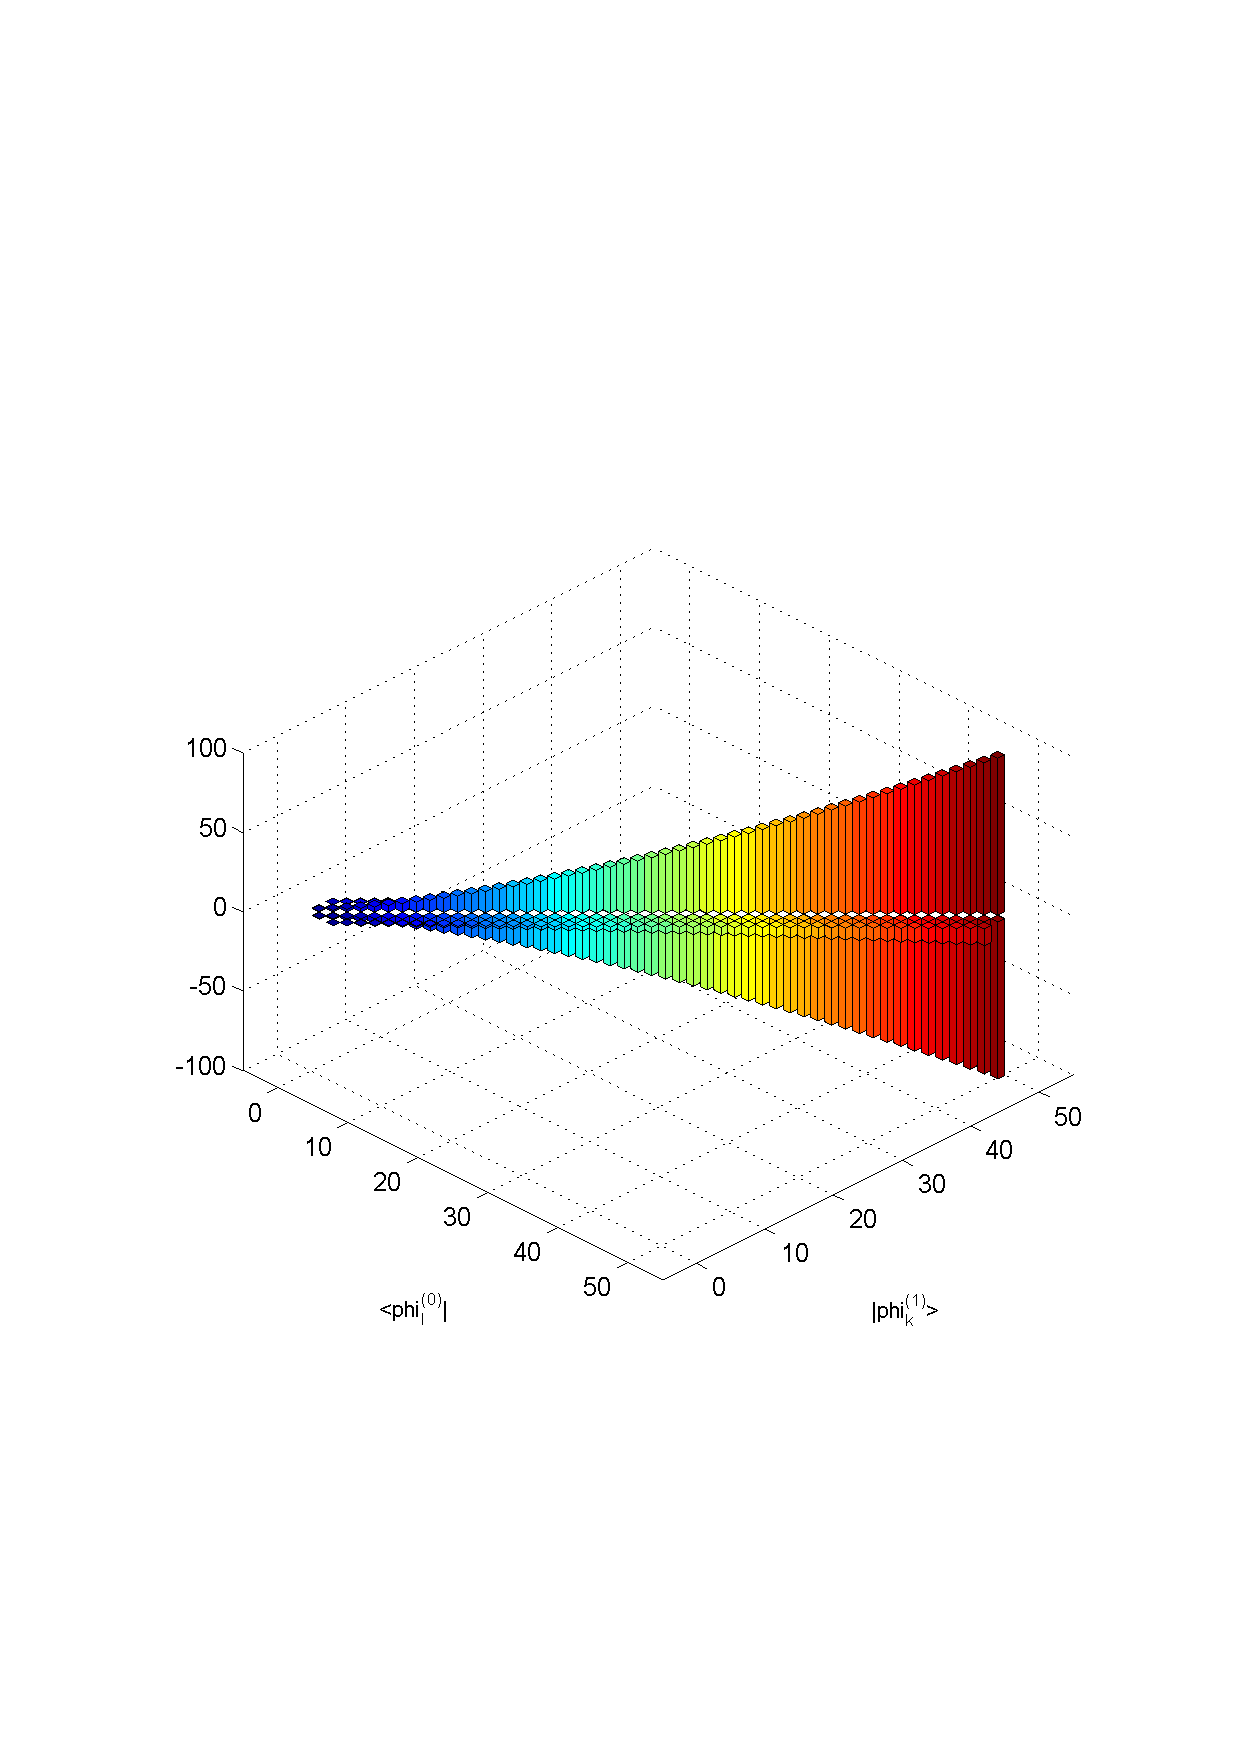
\includegraphics[width=0.7\textwidth]{anharmonisch/images/PLK12.pdf}
\caption{Skalare der Wellenfunktionen
\label{skript:PLK12}}
\end{figure}

\[
\Psi_k^{(p)}
=
\imath\gamma|\Psi_l^{(0)}\rangle+
\displaystyle\sum_{l\neq k} \langle\Psi_l^{(0)}|\Psi_k^{(p)}\rangle
|\Psi_l^{(0)}\rangle
\]

\subsection{Auswertung}

\section{Infrarotspektroskopie}
\rhead{Infrarotspektroskopie}
TODO

\printbibliography[heading=subbibliography]
\end{refsection}

